\chapter{Adatok gyüjtése a mesterséges inteligencia betanításához}
\thispagestyle{fancy}
\pagestyle{fancy}


\section{Tervezés}
Ahhoz hogy a mesterséges inteligenciát betanítsuk, szükségünk lesz a lehető legtöbb információra, amit képesek vagyunk egy adott menetről összegyüjteni.
\subsection{Az adatszerkezet}
Egy adott játék a következőképpen néz ki:
\begin{itemize}
\item A játékos az eddigi tudása alapján, kiválasztja melyik sor és melyik oszlop kártyáját választja.
\item Felfordítja a kiválasztott kártyát, ekkor megtudja, milyen betű szerepel rajta. 
\item Ezen információ és az eddigi tudása alapján kiválasztja a következő kártyát a tábláról. Itt két lehetőssége van a játékosnak: 
\begin{itemize}
    \item Tudja vagy legalábbis nagy százalék valószínűséggel sejti, hogy melyik a párja a kártyának 
    \item Egyáltalán nem, vagy kis valószínűséggel tudja, hol a párja, emiatt felfordít direkt olyan kártyát, melyről eddig semmi ismerete nincs. Vagyis ahogy én hívom, felfedezi a pályát.
\end{itemize}
\item Ha párok voltak, eltűnnek a tábláról a kártyák.
\item A játékos ezt a folyamatot addig ismétli, míg el nem tűnik az összes kártya.
\end{itemize}

Amire szükségünk van a játék ismeretéhez tehát a következők: 
\begin{itemize}
    \item Hány kártya van a táblán. Mivel mindig egy $N \cdot N$ négynezetet rakunk ki, így ezt fixen ismerjük. 
    \item Milyen betűk szerepelnek a leosztásban
    \item Sorrendben, melyik sor és oszlop kártyái lettek felfodítva, és mi szerepelt a memória kártyán. 
\end{itemize}

A következő adatszerkezetet fogom használni: 

\begin{figure}[h]
\centering
 \begin{lstlisting}
{
  "data": { 
    "id": "Xx12345"
    "played_games": {
      "6": [
        {
          "card_labels": ['A','B','C','D','E','F'], 
          "card_pair_number": 6,
          "card_selections": [ 
            {
              "chosen_first": true,
              "label": "A",
              "x": 0,
              "y": 0
            },
            {
                ...
            },
          ]
        },
        {
            ...
        }
      ]
    }
  }
}
\end{lstlisting}
\caption{Tanításhoz felhasznált adatszerkezet}
\label{saveJson}
\end{figure}


Magyarázat a \ref{saveJson}. ábrához a következő:
\begin{description}
    \item[id] A játékos ID-je melyet megkap a játék elindításakor. 
    \item[Played\_games] Játszott játékok, ahol a kulcs a darabszáma a kártya pároknak.
    \item[6\:] Egy tömb, ahol az összes játszott játék szerepel, az adott kártyaszámra.
    \item[card\_labels\:] Kártyák lehetséges labeljei. Összes card\_pair\_number darab.
    \item[card\_pair\_number\:] A kártya párok száma, megegyezik a tömb kulcsával. A könnyebb adatkezelés érdekében duplikált adat.
    \item[card\_selections\:] Az összes kártya húzása, a játék előrehaladtával, ez a tömb fog bővülni. 
    \item[chosen\_first\:] Elsőnek lett-e választva. Kiszámolható a kártyaválasztás párosságából.
    \item[label\:] A kártyára írt betű.
    \item[X,Y\:] A kártya sor és oszlop koordinátái.
\end{description}
\subsection{Játék felkészítése}
Ahhoz, hogy a tervek szerint a lehető legtöbb emberhez el tudjam juttatni a játékot, a legkézenfekvőbb megoldásnak láttam, hogy HTML5-be exportáljam ki a játékot. 
Ehhez apróbb átalakításokat kellett végrehajtanom, melyek első sorban vizuálitásban jelentek meg. 

Itt több lehetősségem volt, melyet leszűkítettem kettőre amivel komolyabban foglalkoztam:
Az egyik opcióm, hogy átírom a játékot, és a hozzá tartozó html template-et, mellyel kiexportáltam a játékot, hogy a Weblap javascriptjének segítségével, lementsem a JSON file-t, így azt el tudják majd küldeni nekem, valamilyen online felületen. 
A másik opció, hogy készítek egy file szervert, ahova a JSON-t elküldöm minden sikeres játék után, egy HTTP Request formájában.

Átgondolva a lehetősségeimet, úgy döntöttem, a file szervert választom, megvalósításnak, mivel így biztosan és automatikusan eljut hozzám az összes teszt adat.

A játékhoz készíttem egy  \lstinline{http_client.gd} scriptet, melynek egyetlen feldata volt, hogy egy  \lstinline{HTTP POST} kérést küldjön el egy weboldalnak. A HTTP request body részébe beraktam a JSON file. Ezt a scriptet minden játék befejeztével aktiváltam. 

Ahhoz, hogy a kérés mindig sikeres legyen, muszáj volt megcsinálnom, hogy az ha egy játékosnak nincs ID-je, akkor ha üresen hagyja a beviteli mezőt, egy random generált ID-t kapjon. Az ID-t a menü oldalon meg is jelenítettem, és másolhatóvá tettem. 
A játék állását, vagyis azt, hogy melyik játékkal mennyit játszott a játékos, azt a lokális böngésző IndexedDB-jébe menti a Godot automatikusan. Így ha egy játékos akkor játszik, mikor éppen nem elérhető a szerver, később is el tudja küldeni a játszott játékainak statisztikáját.
\begin{figure}[h]
    \centering
    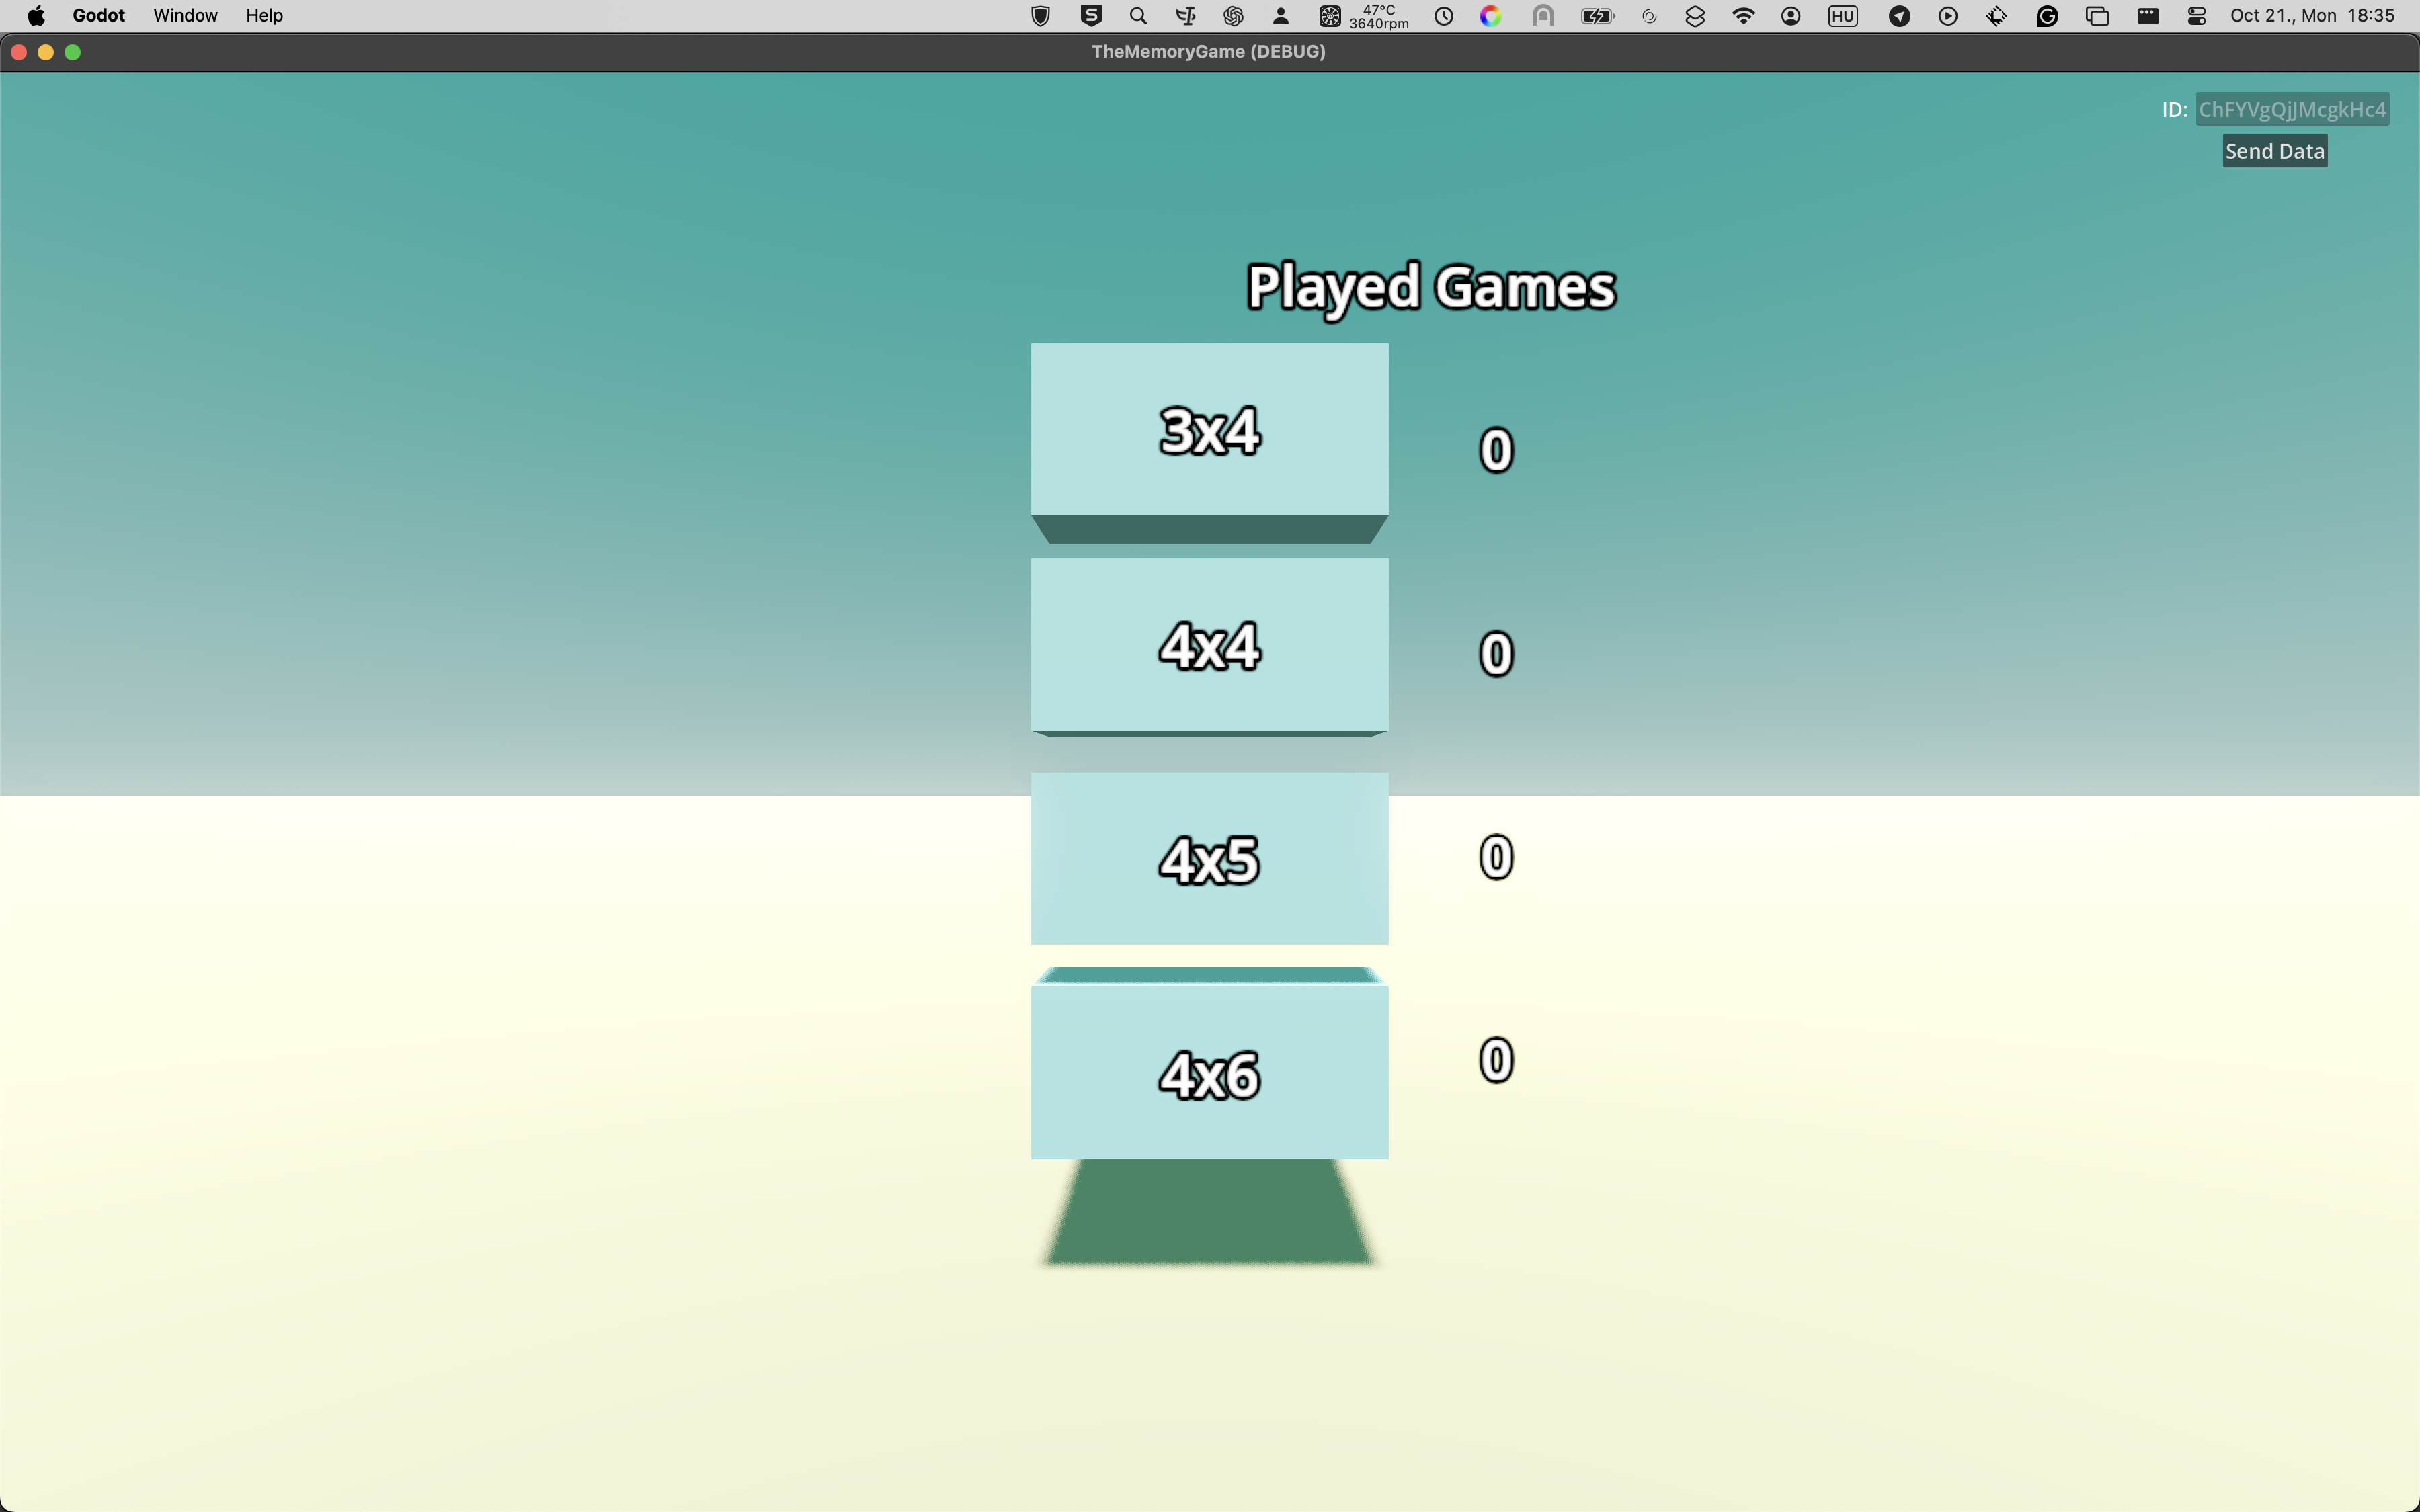
\includegraphics[width=0.75\textwidth]{img/menu_remake.png}
    \caption{Az átlakaított menü: másolható ID mező, és egy küldés gomb}
    \label{img:menu_remake}  
\end{figure}

\section{File szerver megvalósítása}
A fájlszerver megvalósításához JavaScriptet és NodeJS-t használtam.
A szerver működtetésére az Express web framework-öt vettem igénybe, 
A fájlszerver egyetlen végpontot biztosított, amely a \lstinline{/save_json} útvonalon volt elérhető. 
Ez a végpont fogadta az érkező JSON formátumú adatokat, és a szerver feladata volt ezeknek az adatoknak a fájlrendszerbe történő mentése. 
A mentési folyamat során az adatok az ID szerint kerültek elhelyezésre külön mappákba, ahol a mappa neve a játékos ID-ja volt. 
Az egyes mappákban az aktuális időpont szerint elnevezett JSON fájlok kerültek tárolásra, például: \texttt{2023-10-21T12:34:56.json}. 
Ez a struktúra biztosította az adatok könnyű visszakereshetőségét és rendszerezhetőségét.

Annak érdekében, hogy a szerver domain néven keresztül is elérhető legyen, a Cloudflare Tunnel szolgáltatást alkalmaztam. 

A rendszer kényelmes használata és virtuális gépen történő telepítése érdekében a szervert és a Cloudflare-t is külön-külön Docker konténerben futtattam.
A konténerek használata egyszerűvé teszi a telepítést és a menedzselést, mivel az alkalmazások és azok függőségei elszigetelten futnak. 
A Docker Compose segítségével pedig könnyedén integrálhattam és menedzselhettem a többkonténeres alkalmazásokat, ami lehetővé tette a szerver és a Cloudflare Tunnel együttes futtatását és összehangolt működését.

\begin{figure}[h]
    \centering
\begin{lstlisting}
services:
file-server:
  build:
    context: .
  volumes:
    - ./data:/app/data
cloudflair:
  image: cloudflare/cloudflared:latest 
  command: tunnel --no-autoupdate run --token <token>
\end{lstlisting}
\caption*{docker-compose.yaml}
\label{code:docker-compose}
\end{figure}
\begin{figure}[h]
    \centering
    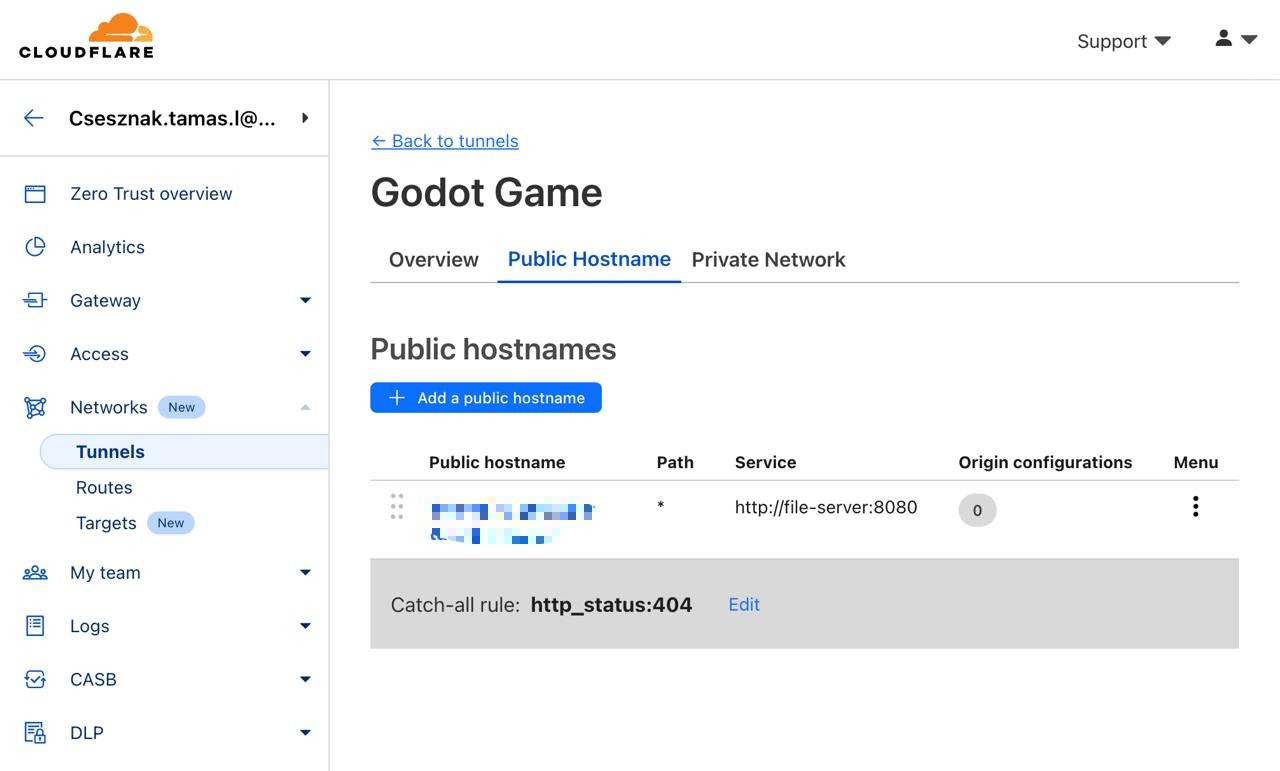
\includegraphics[width=0.75\textwidth]{img/cloudflair-censored.jpg}
    \caption{Cloudflair tunne konfiguráció}
    \label{img:cloudflair-config}  
\end{figure}


\subsection{Oracle Cloud}
A fájlszerver telepítéséhez először az Oracle VM-et szerettem volna használni. Az Oracle VM egy rendkívül megbízható és skálázható megoldás, amely lehetővé teszi, hogy virtuális gépeket hozzunk létre és futtassunk különböző platformokon. Az Oracle VM számos előnnyel rendelkezik, mint például a magas teljesítmény, a robusztus biztonsági funkciók, és a kiváló támogatás. Ezen kívül számos operációs rendszerrel kompatibilis, ami megkönnyíti a különféle alkalmazások és szolgáltatások telepítését és futtatását.

Az Oracle VM-en keresztül kívántam a fájlszerveremet üzemeltetni, mivel reméltem, hogy a szolgáltatás rugalmassága és skálázhatósága előnyös lesz a projekt szempontjából. Az Oracle VM felületén könnyedén konfigurálhatók a virtuális gépek, és a hálózati beállítások is egyszerűen kezelhetők. Emellett a szolgáltatás integrálhatósága más Oracle termékekkel és szolgáltatásokkal további előnyöket kínál.

Azonban, amikor megpróbáltam igénybe venni az Oracle VM ingyenes erőforrásait, sajnálatos módon azt tapasztaltam, hogy ezek nem voltak elérhetők. Az ingyenes erőforrások hiánya miatt kénytelen voltam alternatív megoldást keresni, mivel nem tudtam megfelelően kihasználni az Oracle VM által nyújtott lehetőségeket. Ez komoly csalódást okozott, mivel úgy gondoltam, hogy az Oracle VM ideális lenne a fájlszerverem futtatására, de az ingyenes hozzáférés hiánya miatt további megoldásokat kellett keresnem.


\subsection{Fly.io}
Miután az Oracle VM nem bizonyult járható útnak, úgy döntöttem, hogy kipróbálom a Fly.io szolgáltatását. A Fly.io egy modern felhőalapú platform, amely lehetővé teszi az alkalmazások globális szinten történő futtatását és skálázását. A szolgáltatás fő célja, hogy az alkalmazásokat közelebb hozza a felhasználókhoz, ezáltal csökkentve a késleltetést és javítva a teljesítményt. A Fly.io platformja rendkívül egyszerűen használható, és számos automatizált funkcióval rendelkezik, amelyek megkönnyítik az alkalmazások telepítését és kezelését.

A Fly.io honlapja első ránézésre ígéretesnek tűnt, és úgy tűnt, hogy ingyenes használati lehetőséget is kínál. Ez különösen vonzó volt számomra, mivel szerettem volna minimalizálni a költségeket a projekt korai szakaszában. A Fly.io segítségével könnyedén létrehozhattam és kezelhettem a fájlszerveremet, és a platform egyszerűsége miatt gyorsan és hatékonyan tudtam dolgozni.

Azonban, amikor elkezdtem a fájlszerver telepítését és k
onfigurálását a Fly.io platformján, kiderült, hogy a szolgáltatás nem teljesen ingyenes.
A Fly.io használatával kapcsolatos üzenetváltások darabszámára vonatkozó díjak jelentősen 
megnövelték volna a költségeket. Ez komoly kihívást jelentett, és nem számítottam ilyen jellegű kiadásokra. 
Az ingyenesnek tűnő szolgáltatásról kiderült, 
hogy valójában nem az, ami csalódást okozott, 
és újra arra kényszerített, hogy más megoldásokat keressek a fájlszerverem üzemeltetéséhez.

Mindkét esetben a szolgáltatások ígéretes lehetőségeket kínáltak, de végül nem feleltek meg az elvárásaimnak az ingyenes erőforrások és a rejtett költségek miatt. Azonban a tapasztalatok segítettek abban, hogy jobban megértsem a különböző felhőalapú platformok működését és költségstruktúráját, ami hasznos lesz a jövőbeni projektek tervezésénél és megvalósításánál.
\section{Végleges megoldás}
Mivel sajnos nem találtam más alternatívát, ami ingyenes lenne, így kénytelen voltam a helyi gépemen futtatni a docker containereket, és megkérni a játék tesztelőket, hogy akkor futtassák a játékot, amikor éppen üzemel a file szerver. 